\subsection{PDF Signature Spoofing}
Die PDF-Spezifikation ist sehr ungenau, im Bezug auf digitale Signaturen bzw. auf welche Art und Weise sie validiert werden müssen. PDF-Viewer haben eine hohe Toleranz beim Öffnen, Validieren und Anzeigen von beschädigten PDF-Dateien. Im Jahr 2019 wurden 3 Attacken zum Vortäuschen von validen PDF-Signaturen erforscht: \gls{isa}, \gls{swa} und \gls{usf}. Das attack scenario sieht wie folgt aus: Der Angreifer besitzt das signierte PDF mit einer gültigen digitalen Signatur und manipuliert es. Das manipulierte, signierte PDF wird an das Opfer geschickt und die Signatur bleibt gültig, obwohl der Inhalt geändert wurde. Die \gls{isa} nutzt das incremental update-Feature von PDF aus, um bösartigen Inhalt in das PDF des Opfers zu schleusen. Im Prozess des Signierens wird ein incremental update verwendet, um die Signatur zu speichern. Am Ende des Originaltrailers wird ein neuer Katalog und ein neues Signatur-Objekt als Body Updates angehängt, was den Signaturwert und Informationen über den Ersteller der Signatur enthält. Danach wird eine updated Xref section und ein updated Trailer angehängt. Beim inremental update können Objekte mit anderem Inhalt neu definiert werden. Bei einem spezifikationskonformen incremental update wird der updated Body hinter dem Originaltrailer dem Dateiende hinzugefügt. Darunter zeigt die updated Xref section auf das neue Objekt und der updated Trailer wird ganz am Ende angefügt. Abbildung \ref{fig:incr-update} zeigt den Vorgang des Speicherns einer digitalen Signatur mittels incremental update.

\begin{figure}[!htbp]
	\centering
	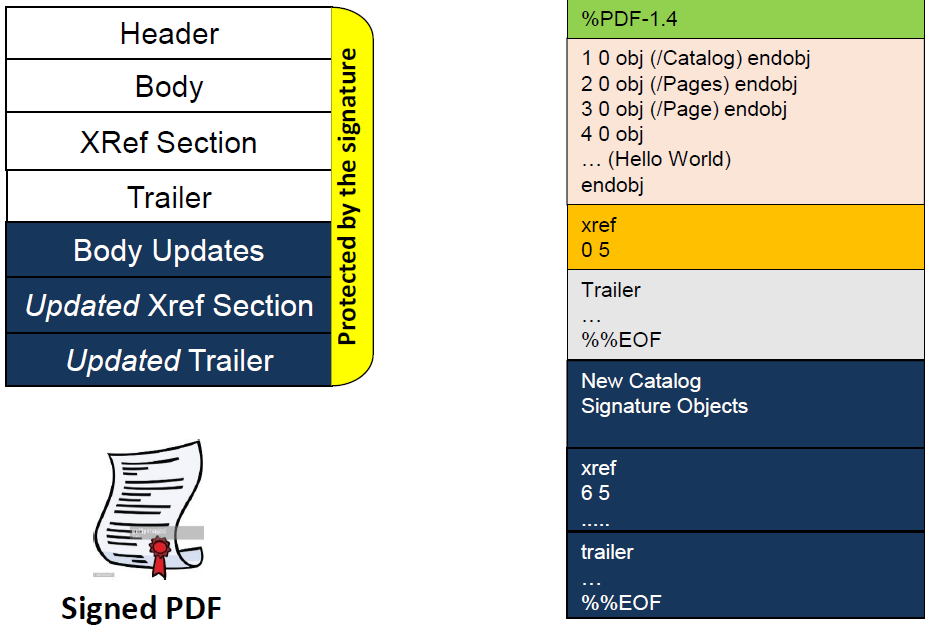
\includegraphics[width=0.8\textwidth]{"images/dig_sig_incr_up.png"}
	\caption{Incremental update mit digitaler Signatur \cite{ccc-break-pdf-slides}}
	\label{fig:incr-update}
\end{figure}

Als erstes hat man bei der \gls{isa} geprüft, ob die PDF-Reader gegen folgende Attacke anfällig sind: Unter dem incremental update mit digitaler Signatur hat man eine weitere Sektion mit Body Updates, Xref und Trailer angefügt. Ausschließlich LibreOffice wurde mittels dieser Vorgehensweise getäuscht. Alle weiteren Strategien produzieren beschädigte, nicht standardkonforme PDF-Dateien, jedoch PDF-Viewer sind sehr fehlertolerant. Als Nächstes haben die Forscher hinter dem updated Trailer des incremental updates der Signatur Body Updates hinzugefügt. Einige getestete PDF-Viewer haben lediglich überprüft, ob neue Xref und Trailer vorhanden sind. Da sie fehlten, blieb die Signatur gültig, die zusätzlichen Body Updates wurden ausgeführt und die Modifikation blieb ohne Warnung unbemerkt. Andere PDF-Viewer benötigten, neben zusätzlichen Body Updates, noch einen Trailer ohne Xref dazwischen, damit keine Warnung geworfen wird. Die komplexeste Vorgehensweise, bei der neue Body Updates mit einer Kopie des Signatur-Objekts am Dateiende angebracht wurde, hat einige PDF-Viewer wie Foxit gezwungen die Signatur 2 Mal zu validieren. Als Ergebnis wurden die Body Updates erfolgreich eingefügt. In der Grafik \ref{fig:isa} werden die Techniken visualisiert, sowie die PDF-Viewer dargestellt, die anfällig für die genannten \gls{isa}-Vorgehensweisen sind.

\begin{figure}[!htbp]
	\centering
	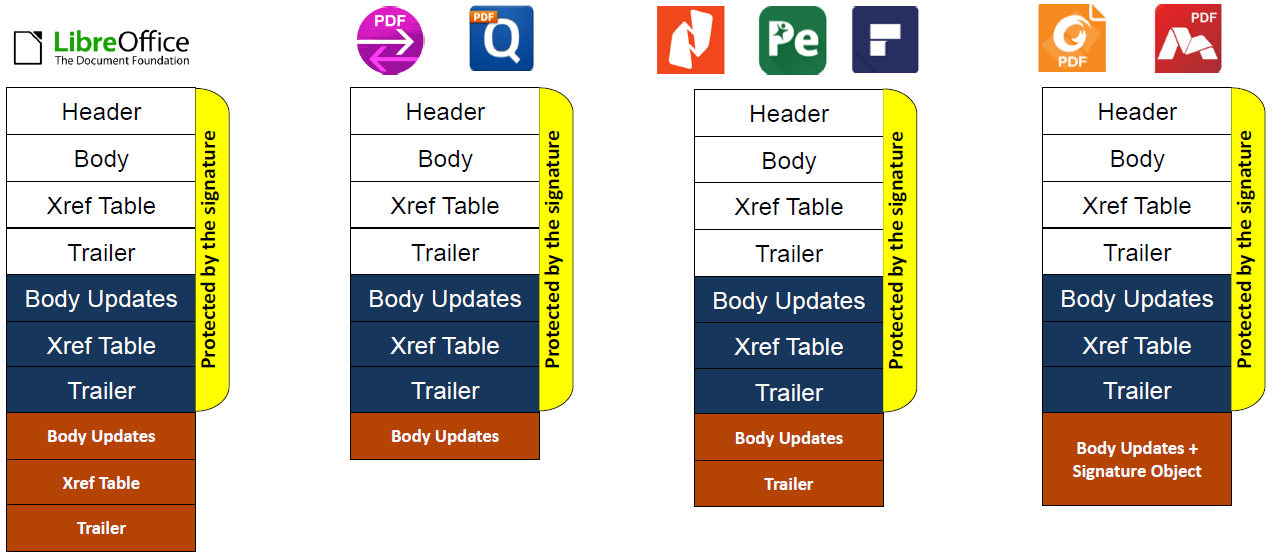
\includegraphics[width=0.8\textwidth]{"images/isa.png"}
	\caption{\gls{isa}-Methoden mit anfälligen PDF-Viewern \cite{ccc-break-pdf-slides}}
	\label{fig:isa}
\end{figure}

Bei der \gls{swa} werden die Werte der signierten /ByteRange modifiziert und Platz wird für das Einschleusen von bösartigen Inhalten geschaffen. Das Signatur-Objekt besteht aus einem /Contents entry mit dem Signaturwert und einem /ByteRange entry mit 4 Werten, welcher den signierten Teil im Dokument anzeigt. Die ersten 2 Einträge der /ByteRange beziehen sich auf den Beginn des Dokuments bis zum Anfang des Signaturwerts. Hingegen definieren die letzten beiden ByteRange-Einträge den Bereich nach dem Signaturwert bis zu \%\%EOF. Diese beiden Bereiche bleiben unverändert. Die erfolgreiche Idee war, eine zweite /ByteRange hinter dem Signaturwert mit einem angepassten dritten Wert, der Platz für bösartige Objekte schafft, etwas Padding und eine bösartige Xref, die auf die Objekte des Angreifers zeigt, zu setzen. Lediglich die Position der neuen Xref ist im Trailer vorgegeben, der nicht verändert werden kann. Das Schaubild \ref{fig:swa} zeigt, wie die \gls{swa} arbeitet.

\begin{figure}[!htbp]
	\centering
	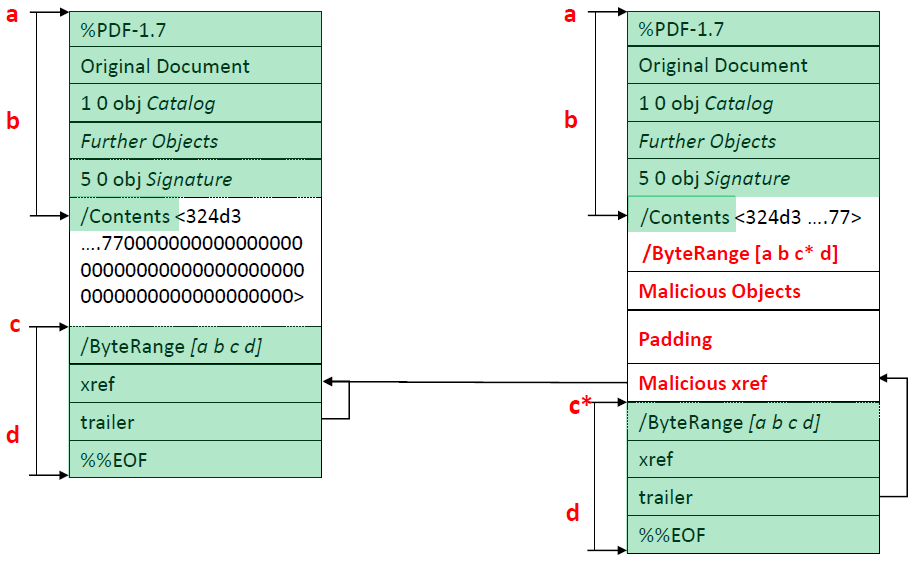
\includegraphics[width=0.8\textwidth]{"images/sig_wrap_attack.png"}
	\caption{\gls{swa}-Methodik \cite{ccc-break-pdf-slides}}
	\label{fig:swa}
\end{figure}

Mittels \gls{usf} wird die Signaturvalidierung außer Kraft gesetzt. Dennoch wird die Meldung – PDF is validly signed – dem Benutzer angezeigt. Vor allem die Adobe-Produkte waren anfällig für diese Attacke. Die Vorgehensweise gestaltete sich wie folgt: Die Forscher versuchten /Contents oder /ByteRange der Signatur entweder wegzulassen oder unübliche Werte, wie kein Wert oder null zuzuweisen. Zwei PDF-Viewer versagten, als man /Contents auf 0 Bytes setzte. Das Weglassen der /ByteRange oder das Gleichsetzen mit null brach die Sicherheitsmechanismen von Adobe. Die Grafik \ref{fig:usf} zeigt die \gls{usf}-Varianten, die von den Forschern getestet wurde.

\begin{figure}[!htbp]
	\centering
	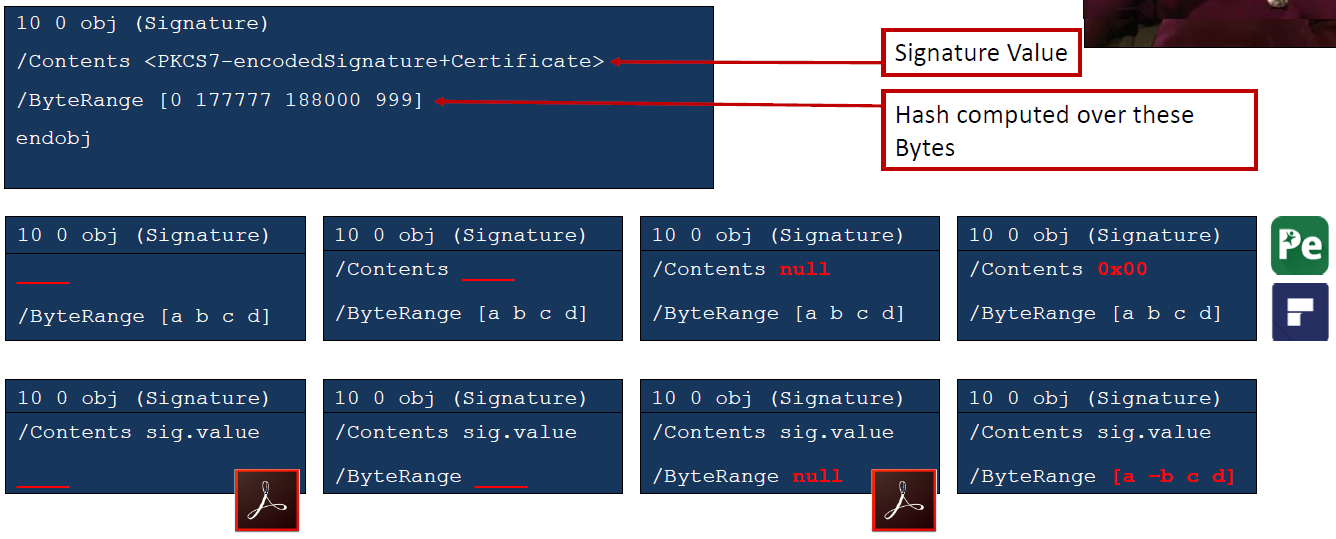
\includegraphics[width=0.8\textwidth]{"images/univ_sig_forgery.png"}
	\caption{\gls{usf}-Varianten \cite{ccc-break-pdf-slides}}
	\label{fig:usf}
\end{figure}

Mittels dieser Attacken ist es den Forschern gelungen zu zeigen, dass 21 von 22 PDF-Viewer, inklusive denen von Adobe, und 6 von 8 Online-Anbieter anfällig sind. Der einzige PDF-Viewer, der gegen alle Attacken immun ist, ist die veraltete Version von Adobe Reader 9, die jedoch remote code execution enthält \cite{ccc-break-pdf}. 